\scanpage{298}
\diagram{\begin{tikzcd}[ampersand replacement=\&,row sep=small,column sep=small]
\& X_1\amalg_Y X_2 \&\\
X_1\arrow[ur] \& \& X_2\arrow[ul]\\
\& Y\arrow[ul,"\varphi_1"']\arrow[ur,"\varphi_2"] \&
\end{tikzcd}}

\diagram{\begin{tikzcd}[ampersand replacement=\&,row sep=small]
X_1\amalg_Y X_2 \&\\
X_1\amalg X_2\arrow[u]\arrow[r,dash] \& {}\\
Y\arrow[u,shift left]\arrow[u,shift right] \&
\end{tikzcd}}

Contre-exemples par \deleted{\unsure{reco}}\inserted{recollement}

$\varphi_i$ immersions

\[
\begin{aligned}
\text{\uline{exemple 1}} \qquad X_1=X_2&=\overbrace{\operatorname{\unsure{Spectre|Spec}} k[x,y]}^{\deleted{\unsure{Z|X}}X}-\text{origine}\\
\deleted{Y=\underbrace{\operatorname{Spec}k[t]}_{Z}-\text{origine}}&=\operatorname{Spec} k[t,t^{-1}]
\end{aligned}
\]

$\varphi_1$ induit par \deleted{\illegible{1}} $\deleted{Y}Z\to X$ défini par les équations : \quad $x=\deleted{\unsure{1/x}}t$, $y=0$

\figure{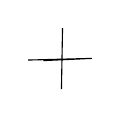
\begin{tikzpicture}[x=1em,y=1em]\draw (0,-1.05)--(.04,1.15);\draw (-1.2,0)--(1.1,.06)--(-.65,-.02);\end{tikzpicture}}

\[
\begin{aligned}
&\deleted{\varphi_2\qquad Z\to X}\\
&\deleted{\hspace{8em}x=1/\unsure{.|t}}\\
&\deleted{\varphi_2\unsure{\varphi_2|\psi}=\varphi_1\psi\qquad\div\quad\psi}\\
&\hspace{8em}x=1/t,\quad y=0
\end{aligned}
\]

$X'=X_1\amalg X_2$ est \unsure{quasi-affine}

$X=X_1\amalg_Y X_2$ ne l'est pas, car

$\Gamma(X,\underline O_X)={}$ \deleted{\unsure{ensemble}} \unsure{sous-anneau} de $\Gamma(X')$ formé des $(f_1,f_2)$ \unsure{telles|tels} que $f_1\deleted{\unsure{(t,0)}}\circ\varphi_1=f_2\circ\varphi_2$. Or $\Gamma(X_i,\underline O_{X_i})=k[x,y]$, et on a $f_1(t,0)=f_2(1/t,0)$

% archive sheet number: 297

